\section{Energy-Only SuperNEMO Diagnostic}
\label{app:energy-illustration}

\paragraph{Population and operating point.}
This diagnostic uses all 196,608 simulated $0\nu\beta\beta$ and 262,144
$^{214}$Bi events in the existing shared test partitions. It is separate
from the trained $2\nu\beta\beta$ classification task. Energy is the
reconstructed calorimeter sum $E_1+E_2$ in keV, extracted once per event;
the identical event-level fields repeated on tracker rows are not counted
as separate observations. The released two-electron topology selection
applies, with no additional energy cut or random sampling for the spectra.
Class normalization removes differences in simulation sample counts; it
does not estimate exposure-normalized physical rates.

\begin{figure}[!htb]
\centering
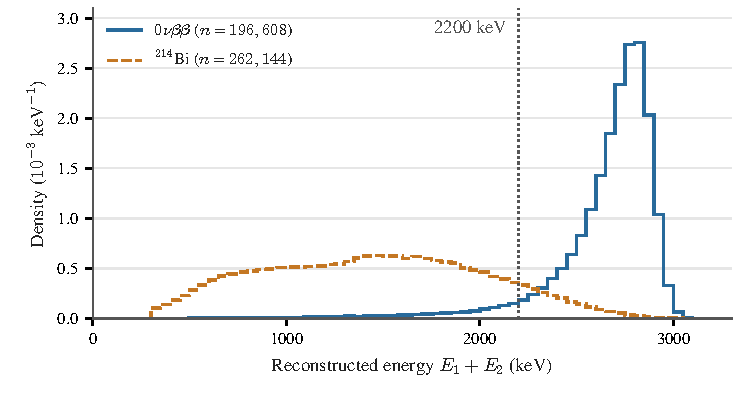
\includegraphics[width=.90\linewidth]{wing_contribution/figures/energy_bias_spectrum.pdf}
\caption{The motivating energy-spectrum difference: 196,608 simulated
$0\nu\beta\beta$ and 262,144 $^{214}$Bi events from shared SuperNEMO test
partitions. The 50\,keV display bins have unit area per class, so sample
counts do not determine their relative heights. The released two-electron
selection applies \citep{macko2026supernemo}; no additional energy cut is
applied to the plotted spectra. The vertical line marks the illustrative
2200\,keV threshold, not a test-optimized operating point.}
\label{fig:supernemo-energy-spectrum}
\end{figure}


At the illustrative threshold $t=2200$\,keV, the rule
$\widehat y_i=\mathrm{1}\{E_i\geq t\}$ accepts 184,727 of 196,608 signal
events and 26,793 of 262,144 background events. Hence
\begin{equation}
 \mathrm{TPR}=0.939570,\qquad \mathrm{FPR}=0.102207,\qquad
 \mathrm{BA}=\tfrac12[\mathrm{TPR}+(1-\mathrm{FPR})]=0.918681,
\end{equation}
where BA is balanced accuracy, assigning equal importance to both classes.
Figure~\ref{fig:energy-threshold} shows the operating-point trade-off.
The threshold was specified for illustration rather than selected by
maximizing test performance. Neither this cut nor the score $s_i=E_i$
requires training or event topology.

\begin{figure}[!htb]
\centering
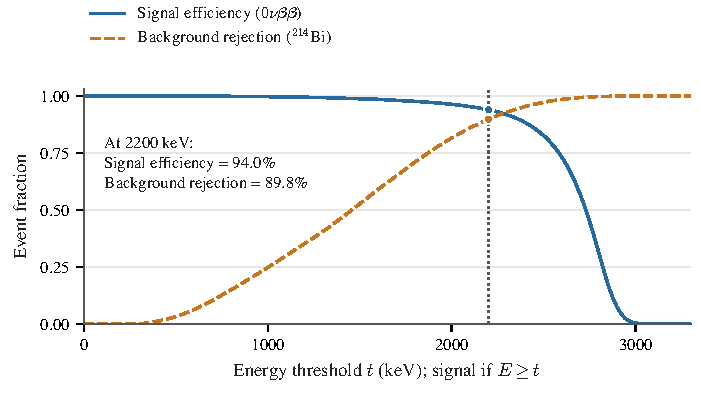
\includegraphics[width=.85\linewidth]{wing_contribution/figures/energy_threshold_tradeoff.pdf}
\caption{Signal efficiency and background rejection as an energy-only
threshold varies in the same SuperNEMO $0\nu\beta\beta$--$^{214}$Bi test
partitions. Curves use all events; the display samples thresholds every
10\,keV. Markers identify the illustrative 2200\,keV cut, with rates
calculated directly from event energies.}
\label{fig:energy-threshold}
\end{figure}

\paragraph{Matching and coverage.}
We apply the shared 600 regular 5\,keV bins plus one overflow bin to this
diagnostic pair, with
class-wise 0.5\% tail trimming, overlap matching, and at least 20 events
of each class per bin. Common support remains
$C=[1169.390,2734.195]$\,keV. The slice of the zero-anchored grid
intersecting $C$ has edges
\begin{equation}
 (1165,\ 1170,\ 1175,\ \ldots,\ 2730,\ 2735)
 \;\mathrm{keV}.
\end{equation}
Events must also satisfy $E\in C$, so the boundary bins are partially
occupied. Of 314 candidate bins, 283 pass the count requirement; sparse
bins are excluded without merging. This retains 99,139 signal and
150,591 background events, or fractions 0.504247 and 0.574459, respectively.
Both satisfy the minimum coverage of 0.5, with signal coverage close to
the boundary. The matched result therefore describes the retained energy
population, not the full signal peak. Reweighting gives effective sample
sizes of approximately 34,127 and 64,317. The 50\,keV display bins in
Figures~\ref{fig:energybench-auc}(a,b) and
\ref{fig:supernemo-energy-spectrum} do not set the matching resolution.

The inclusive ROC uses all original energies. The shared energy grid is
assigned before support trimming, including 758 signal and 40 background
events with $E>3000$ keV in one overflow bin. All energies are finite and
nonnegative. Here $C$ lies below 3000 keV, so overflow events receive zero
matched weight; they remain in the coverage denominators and in the
separate independence calculation whenever the group/bin count rule passes.
No energies are clipped. The trained $2\nu\beta\beta$ task uses the same
evaluation rules on its own distinct test population.

\begin{table}[h]
\centering
\small
\caption{Energy-only AUC under successive evaluation conditions. Retained
event counts are unweighted; only the last row uses matching weights.
The populations and weights differ, so these rows are not competing models.}
\label{tab:energy-only-stages}
\begin{tabular}{lrrr}
\toprule
Evaluation condition & Signal events & Background events & AUC \\
\midrule
Original test populations & 196,608 & 262,144 & 0.970613 \\
Common support, unit weights & 99,595 & 172,757 & 0.934642 \\
Retained 5\,keV bins, unit weights & 99,139 & 150,591 & 0.929715 \\
Retained 5\,keV bins, matched weights & 99,139 & 150,591 & 0.500024 \\
\bottomrule
\end{tabular}
\end{table}

\paragraph{Residual within-bin ordering.}
For the increasing score $s=E$, let $q_k$ denote the shared matched mass
of ordered energy bin $k$, and let $A_k$ be the energy-only AUC within that
bin, with half credit for ties. Cross-bin comparisons give
\begin{equation}
 \operatorname{AUC}_{\mathrm{match}}(E)
 =\sum_{k>\ell}q_kq_\ell+\sum_kq_k^2A_k
 =\frac12+\sum_kq_k^2\left(A_k-\frac12\right).
 \label{eq:energy-only-decomposition}
\end{equation}
Equal bin masses balance cross-bin pairs, while within-bin energy
differences remain. This identity gives AUC 0.500024 for the fixed
5\,keV matching bins;
it does not redefine the metric as an average of per-bin AUCs. A score
depending only on bin identity would instead have matched AUC exactly
$1/2$. The independence calculation uses the same energy grid with original base
weights and up to 20 score-quantile bins, yielding $I=0.079210$ for $s=E$.
Its class values are $I_{0\nu}=0.082192$ and $I_{\mathrm{Bi}}=0.076972$.
The 337 and 514 eligible group bins retain 195,169 signal and 261,873
background events, respectively, including their eligible overflow bins.
The energy-only score still varies within each 5 keV bin; balanced bin
masses therefore do not imply exact continuous-score AUC $1/2$.
These are deterministic diagnostic values, without
bootstrap intervals or multiple-seed averages. They demonstrate the
availability of an energy-only decision rule, not the internal strategy
of any trained model or a measured failure under distribution shift.
